\chapter{A look into the codes} \label{ch:lookinto}

in this chapter the code will be explained.

\section{Include files} 

The compiler will always look through the first lines before doing anything else. This is why it is needed to include all the files that is wanted, in the code, in the first lines.\\

\begin{figure}[h]
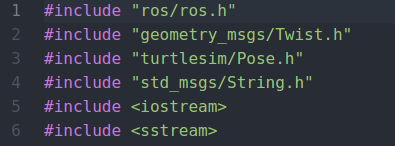
\includegraphics[width=.5\textwidth]{figures/therealinclude.png}
\end{figure}\label{fig:include}

\begin{itemize}
\item \texttt{ros/ros.h}\\
this is a header to include all headers necessary for the common pieces in the ROS system.\\
\item \texttt{geometry\_msgs/Twist.h}\\
includes the headers for the common geometrics as poses, vectors and points.\\
\item \texttt{turtlesim/pose.h}\\
This header file is only needed in the \texttt{Turtlesim\_mover}, since turtlesim/pose is a publisher.\\
This creates the headers for the pose of the virtual turtle.\\
\item \texttt{std\_msgs/String.h}\\
Is a automatized string header, which is generated from the String.msg file.\\
\item \texttt{<iostream>}\\
This is the input/output stream and helps with just that.\\
\item \texttt{<sstream>}\\
Include the std::stringstream.\\

\end{itemize}

\section{The node handler}

\begin{figure}[h]
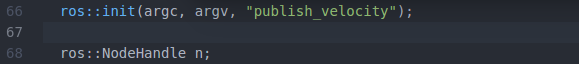
\includegraphics[width=.9\textwidth]{figures/nodehandel.png}
\end{figure}\label{fig:nodehandel}


\section{Publisher}
\begin{figure}[h]
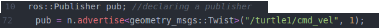
\includegraphics[width=.9\textwidth]{figures/publisher.png}
\end{figure}\label{fig:publihser}
The publisher needs to be delacerd as variable, it is done by the first line see \ref{fig:publihser}.The next line show what message that is published in this case a geometry::Twist and what topic it is published on /turtle1/cmd\_vel.


\section{Subscriber}
The same as the publisher need a declaration, see \ref{fig:subscriber} 

\begin{figure}[h]
\begin{center}

\includegraphics[width=.9\textwidth]{figures/subscriber.png}
\end{center}
\end{figure}\label{fig:subscriber}

\section{UI\_turtlesim\_mover}

Firstly the include files are introduced.\\
After the include files global parameters are set, such as:\\
\texttt{ros::Publisher pub1;}\\
and\\
\texttt{ros::Subscriber sub1;}\\
and\\
\texttt{string done;}\\
then a void function is made.\\

\begin{figure}[h]
\begin{center}
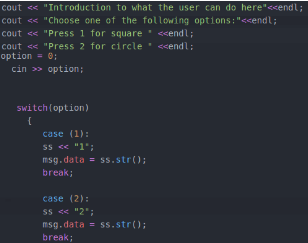
\includegraphics[width=.5\textwidth]{figures/switch.png}
\caption{VoidFunction of UI}
\end{center}
\end{figure}\label{fig:switch}

The void function as seen in \ref{fig:switch}, introduces a series of cout, which will print the text to the users screen.\\
Then the cin option appears. It will determine whether the user will press 1 or 2, and will then store the choice in "Option".\\



\section{Turtlesim\_mover}

\begin{figure}[h]
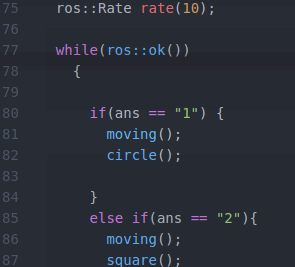
\includegraphics[width=.5\textwidth]{figures/while.png}
\end{figure}\label{fig:while}



\begin{figure}[h]
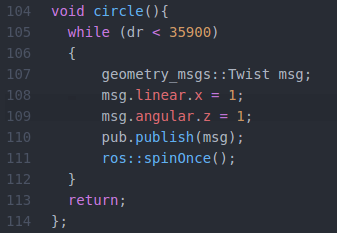
\includegraphics[width=.5\textwidth]{figures/void-circle.png}
\end{figure}\label{fig:void-circle}
